
\documentclass[12pt]{article}

\usepackage{graphicx}
\graphicspath{ {./images/} }

\usepackage{epsfig}
\usepackage{amsmath,amsthm}
\usepackage{listings}


\newtheorem{lemma}{Lemma}
\newtheorem{theorem}{Theorem}


\usepackage{titlesec}
\titleformat{\section}
{\normalfont\Large\bfseries}{Question~\thesection:}{1em}{}

\newlength{\toppush}
\setlength{\toppush}{2\headheight}
\addtolength{\toppush}{\headsep}


\def\subjnum{Comp 160}
\def\subjname{Algorithms}


\def\doheading#1#2#3{\vfill\eject\vspace*{-\toppush}%
  \vbox{\hbox to\textwidth{{\bf} \subjnum: \subjname \hfil Erli Cai}%
    \hbox to\textwidth{{\bf} Tufts University, Fall 2020 \hfil#3\strut}%
    \hrule}}


\newcommand{\htitle}[1]{\vspace*{1.25ex plus 1ex minus 0ex}%
\begin{center}
{\large\bf #1}
\end{center}} 

\setlength\parindent{0pt}


\begin{document}
\doheading{2}{title}{Homework 07}

\section{Magical Stones}
a.(i) stones:[4], so at least 1 stone is needed\\
(ii) stones: [24,24,24,24,24,24,24,17,17,1], so at least 10 stones is needed\\
(iii) stones: [5,5,5,7,7,7] so at least 6 stones is needed\\

b(i) MS(c,0) = 0, MS(c, k) = (No solution) for all $k < 0$\\
(ii) we have to recurse on MS(c, k) for all $k > 0$, and k is changing \\
(iii) Suppose c has i elements, them our recurrence formulae would be:


\[
    MS(c,n)= 
\begin{cases}
    \mbox{no solution},& \text{if } n < 0\\
    0 & \text{if } n = 0\\
    1 + min\{MS(c, n-c[0]),... , MS(c, n-c[0])\}         & \text{if } n > 0
\end{cases}
\]

c\\
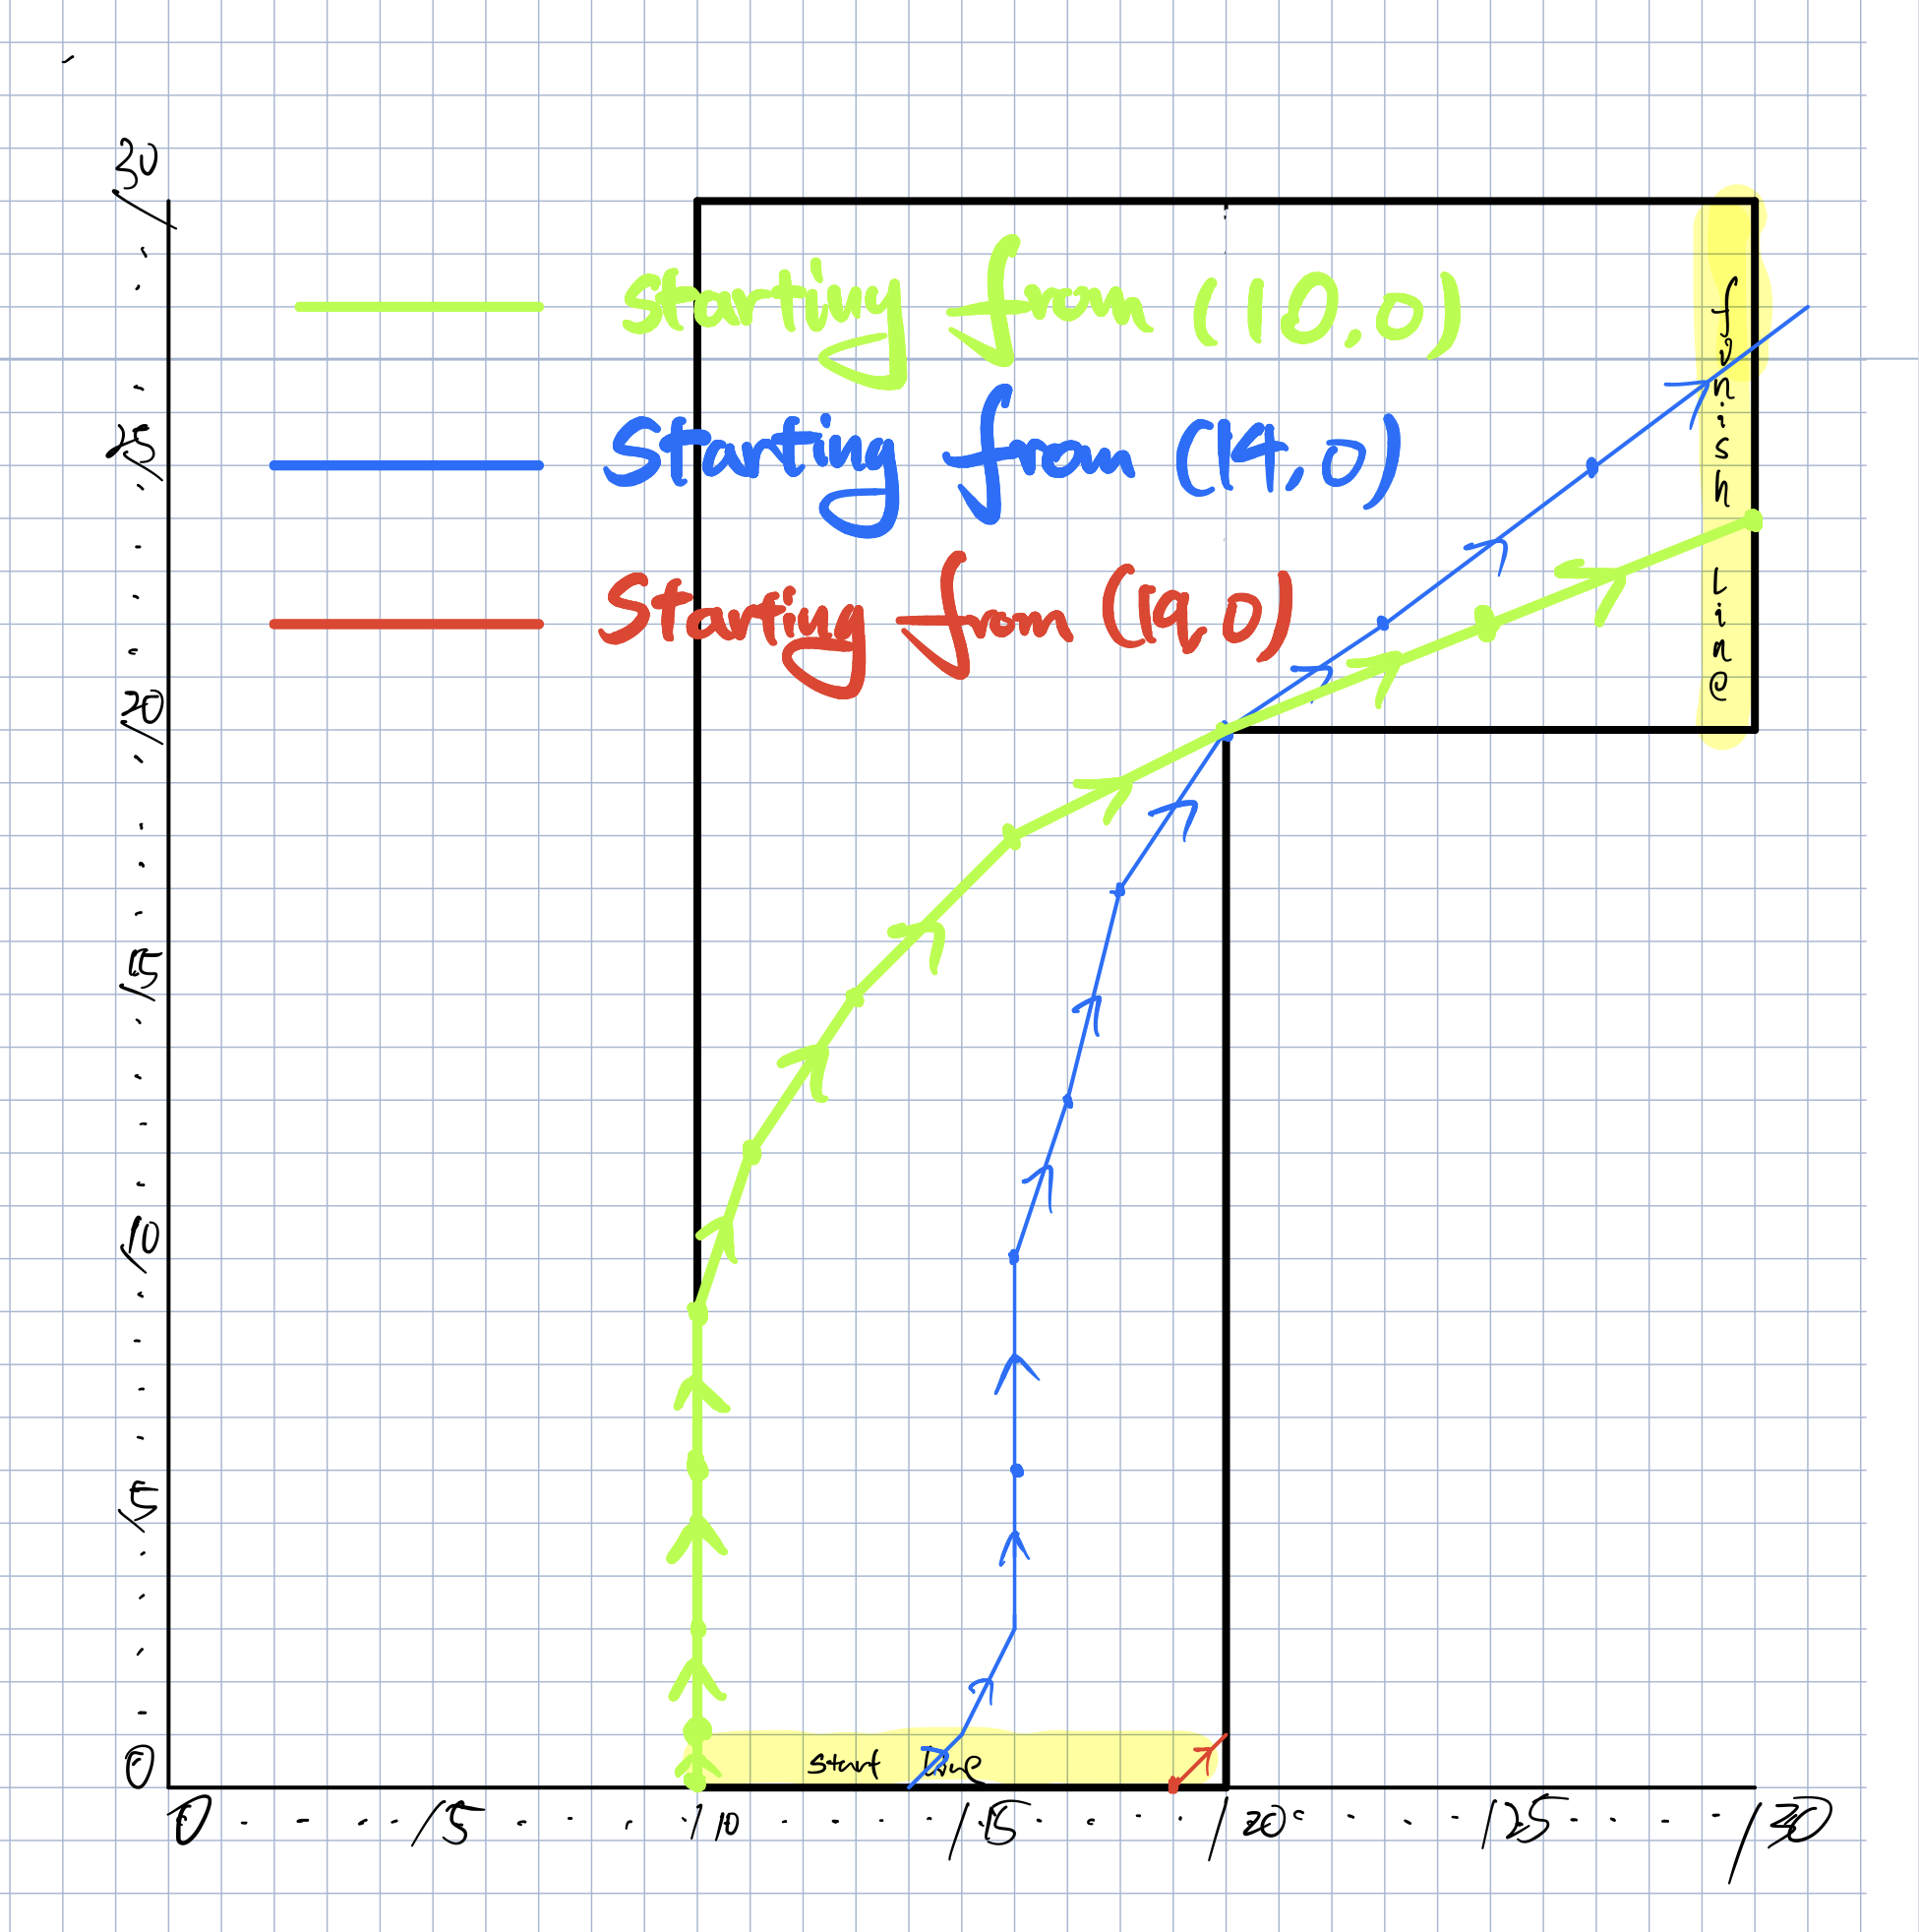
\includegraphics[scale = 0.1]{3.jpg}
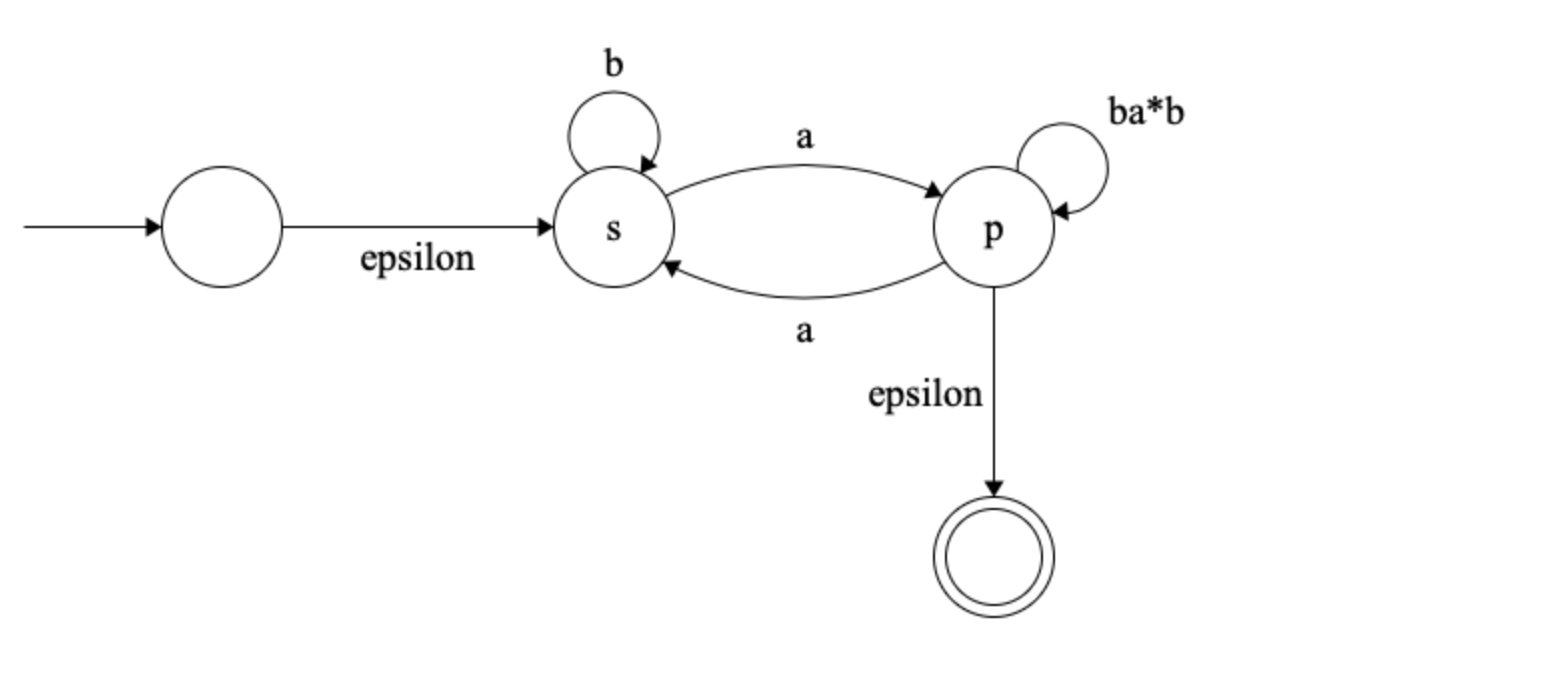
\includegraphics[scale = 0.1]{4.jpg}

d\\
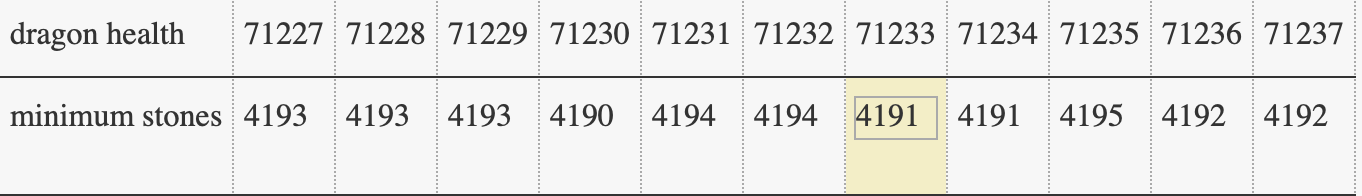
\includegraphics[scale = 0.5]{1}

Given the health of the dragon, say it is n, I will look back to the table where dragon-health = n-3, n-4, n-17. Then the minimum-stones equals to the 1 plus the smallest one of them.


\pagebreak
\section{Health Rituals}


a(i) Casting first and last spell, total healing = 20 + 110 = 130, cost = 15+65 = 80\\
(ii) E = 100 C = [40,50,80]  $\Delta$H = [40,50,81] \\
If choosing greedily, will choose last spell, total heal = 81. But the best solution is choose first 2 spell, total heal = 90.\\

b.
Let  HR(E,C,$\Delta$ H) be a function that takes in energy E, spell cost C and spell healing $\Delta$H\\
Base Case: When the energy is 0 or when there is no spell to case($\delta$H and C are empty), total healing would be 0\\
recursive case: When E is not 0 and  to case, we could either cast the last spell then remaining energy is decreased by C[n], resulting in subproblem $HR(E-C[n],C[1,n-1],\Delta H[1,n-1])$, or not cast it, resulting in subproblem $HR(E,C[1,n-1],\Delta H[1,n-1])$\\
Suppose C and $\Delta$ H has n elements each
\[
    HR(E,C,\Delta H)= 
\begin{cases}
    0  \qquad\qquad\qquad E <= 0\text{ or C and }\Delta H \text{are empty } \\
    \Delta H[n] + max\{HR(E,C[1,n-1],\Delta H[1,n-1]), \\
    \qquad HR(E-C[n],C[1,n-1],\Delta H[1,n-1])\}        & \text{otherwise} 
\end{cases}
\]
\\
c.\\
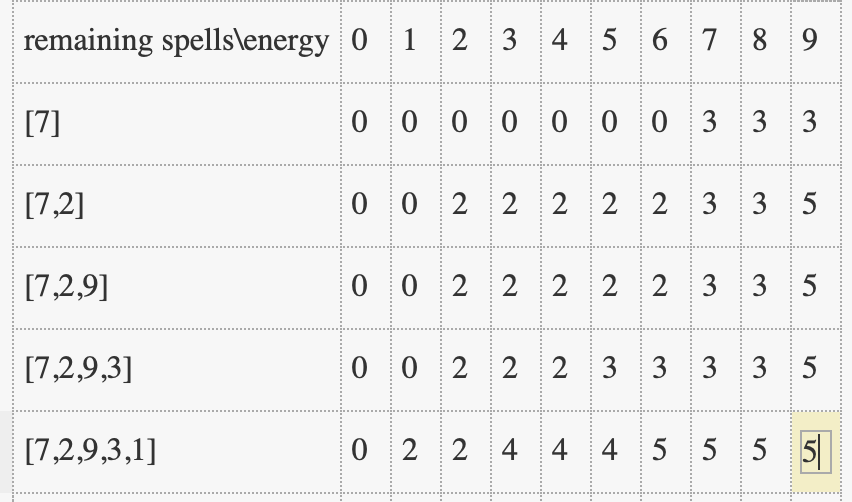
\includegraphics[scale = 0.7]{2}
\\
\pagebreak

d.Suppose C has n elements. subproblems can have energy between 0 and E and spells of length between 1 and n (first  k elements of C).
So we have $\Theta(nE)$ subproblems. Each Subproblem can be computed in O(1) time given that smaller subproblems are already computed. Therefore, The total time and space needed becomes $\Theta$(nE).


\pagebreak
\section{The Secret Code}
Suppose S is a string of length n and Code(S,n) will give us the longest subsequence of palindromes.\\
Base case: 1) n = 0, then longest such string is the empty string, 2) n = 1, then S has only one character and the longest such string is S itself.\\
Recurrence case:  when first character and last character of S are different, recur on first n-1 characters and last n-1 characters, and take the longer one to be the answer. when first character and last character of S are same, recur on S[2,n-1] (from second to second to last character), and the answer is S[1]+ Code(S[2,n-1],n-2) + S[n] (plus sign here represent string concantation).\\
\[
    Coed(S,n)= 
\begin{cases}
    \text{empty string}  &\text{ if } n = 0 \\
    Code(S[2,n-1],n-2)       & \text{if} S[1] = S[n]\\
    max([Code(S[1,n-1],n-1), Code(S[2,n],n-1)] ,key = len)       & \text{if} S[1] != S[n]\\
\end{cases}
\]
\\
Runtime Analysis: Subproblems are consecutive substrings of S, there are $\Sigma_{k=1}^n k = n(n+1)/2 = O(n^2)$ of them, And each subproblem takes O(1) operation if smaller subproblem is already computed. therefore, total runtime is $O(n^2)$



\end{document}







